\documentclass[
    % draft=true,
    paper=a4,
    % mpinclude=true,
    % twoside, % twoside is default for scrbook
    paper=portrait,
    pagesize=auto,
    fontsize=11pt,
    DIV=11, % DIV value as calculated from paper and font size
    % BCOR=15mm, % binding correction
    % titlepage=firstiscover, % print title page as cover
    % version=last,
    % headings=twolinechapter
    ]{scrartcl}

\usepackage{scrhack} % fix a few common issues with KOMA-classes

\setkomafont{disposition}{\rmfamily}
\usepackage{libertinus}
% Citation Management
\usepackage[
    style=authoryear-comp, % citation style
    natbib=true,
    backend=biber,
    maxnames=2,
    maxbibnames=99]{biblatex}
\addbibresource{literature.bib}
\emergencystretch=2em


% while drafting
% \includeonly{sections/introduction}
\setlength {\marginparwidth }{2cm} 
\usepackage[obeyDraft]{todonotes}
\setuptodonotes{inline}

\usepackage[ngerman, english]{babel} %last language in the list is the main language, in this case English (American)
% font as needed for additional languages

% CJK support still best by additional package
\usepackage{xeCJK}
\setCJKmainfont{Noto Serif CJK TC}
\setCJKsansfont{Noto Sans CJK TC}
\setCJKmonofont{Noto Sans Mono CJK TC}
% quotation style
\usepackage[english=american]{csquotes}

% FOR TESTING
\usepackage{blindtext}
% \usepackage{showframe}


% other
\usepackage{graphicx}
\usepackage{hyperref}
\usepackage{caption}
\usepackage{subcaption}


% linguistics stuff
\usepackage{forest}

\begin{document}

% title information
\subject{Proposal for a Master's thesis}
\title{Quantitative typology of valency classes}
\author{Siyu Tao}
\date{Draft as of \today}

\maketitle

\addsec{Abstract}
\blindtext

\section{Introduction}

Argument structure is widely studied and debated in linguistics. The nature of the relationship between verbs and their arguments as well as the syntatic expression of underlying lexical semantics.

\section{Background and Motivation}

\subsection{Valency and valency phenomena}

% valency - terminology introduction

In chemistry, \textit{valency}, or \textit{valence}, refers to the combining power of an atom or radical. The valency of any atom can be measured by the number of hydrogen atoms that it can combine with or displace in a chemical compound \citep{law2020a}. This same term has been used in linguistics to similar effect and refers to the combining power of a word, primarily a verb or other predicate, with other words or elements of the sentence. 

Lucien Tesnière is generally credited with introducing the term valency to linguistics with his syntactic theory of valency and dependence, as presented in the posthumuously published \textit{Éléments de syntaxe structurale} (\cite*{tesniere1959}; English translation \cite*{tesniere2015}).\footnote{
    As \citet{przepiorkowski2018} notes, while Tesnière is rightly credited with the introduction of a theory of linguistic valency, the metaphor of valency itself has made appearances as early as in \citet{peirce1897}, among others.
}
In another of Tesnière's metaphors, each verbal node, being the center of sentence structure, is not unlike a ``theatrical performance'' with the verb expressing the process and the nouns being the \textit{actants} (what we would now call \textit{arguments}) in this performance. Just like atoms of different elements allow for a greater or lesser number of bonds, different verbs can combine with a greater or lesser number of actants, i.e., their valency.

% the phenomena now we are now calling valency - different theories
While the term valency is borrowed into linguistics from chemistry, the study of phenomena that are covered by or overlap with valency has a much longer tradition, dating to the early beginnings of linguistics from the kāraka level of semantic relation between verb and noun \citep{ganeri2011a} in Pāṇinian grammar to modern case grammar \citep{fillmore1967}. 

Most linguistic theories, as well as psycholinguistic evidence, point to the centrality of the verb in determining both the structure and meaning of a sentence. This places valency and the issues of \textit{argument encoding} squarely at the center.

Beyond that, however, approaches to the study of argument encoding differ.

%% generative grammar - subcategorization
In generative grammar, syntactic valency of a verb is studied in terms of ``subcategorization frames'' encoded in the lexicon. \todo{describe Chomskyian approach re subcategorization}

\citet{levin1993}'s seminal work provides much more fine-grained categorization of verbs based on their syntactic behavior. \todo{levin}

%% frame semantics - fillmore 
\citep{fillmore1967,fillmore1970} 


%% construction grammar
CxG would consider valency frame as a level of construction. Whether or not this construction is autonomous will depend on whether the unpredictability condition is satified - in so far that the properties of valency frame cannot be predicted from other grammatical units.

\citet{croft2012} takes a CxG approach. 


\subsection{Cross-lingual and contrastive studies of valency}

% why approach valency from typological perspective
Typological interest in valency is primarily focused on cross-linguistic mismatches.

Already \citet{tesniere1959} describes the process of \textit{metataxis}, by which syntactic structures of one language is translated to those of another.  

\citet{levin2005} identifies five major questions that are necessary for a compelte theory of argument realization.
\todo{copy from hand notes and add how a typological study can help answer some of these questions}

% monolingual valency dictionaries

One of the key question is also whether this valency frame are syntactically defined or semantically so. Since in the study of argument structure, we're dealing with the syntactic expression of lexical and non-lexical semantics, this question is particularly difficult to answer.

% cross-lingual contrastive studies

% typological approaches
\citet{tsunoda1981, tsunoda1985} proposes an hierarchy of verbs



\subsection{Dependency grammars}

Universal Dependencies 




\section{Data and methodology}\label{sec:methodology}

This section presents the proposed data sources and methodology of the thesis. \S\ref{subsec:data-sources} introduces the Universal Dependencies treebanks as well as additional resources that will be used as reference and validation in this study. The rest of the section, \S\ref{subsec:features}-\ref{subsec:infotheory}, presents the main computational methods to be used in the thesis.

\subsection{Data sources}\label{subsec:data-sources}

Universal Dependencies (UD) is designed to be a cross-linguistically consistent system for annotating morphosyntactic information within a dependency grammar framework \citep{demarneffe2021}. The UD treebanks \citep{universaldep} is the collection of cross-lingual treebanks annotated in the UD framework by an open community of more than 300 contributors. See \ref{tab:treebanks} for a table of languages available in UD v2.5, as an example. \todo{include some more statistics of UD and a potential list of languages to study}

\begin{table}[t]{}
    \centering
\begin{adjustbox}{center,scale=0.85}
\footnotesize
\renewcommand{\tabcolsep}{3pt}
    \begin{tabular}{|lrrr|lrrr|lrrr|}
    \hline
    \textbf{Language}  & \textbf{\#} & \textbf{Sents} & \textbf{Words} & \textbf{Language}  & \textbf{\#} & \textbf{Sents} & \textbf{Words} & \textbf{Language}  & \textbf{\#} & \textbf{Sents} & \textbf{Words} \\
    \hline
Afrikaans &1 &1,934 &49,276 &German &4 &208,440 &3,753,947 &Old Russian &2 &17,548 &168,522 \\
Akkadian &1 &101 &1,852 &Gothic &1 &5,401 &55,336 &Persian &1 &5,997 &152,920 \\
Amharic &1 &1,074 &10,010 &Greek &1 &2,521 &63,441 &Polish &3 &40,398 &499,392 \\
Ancient Greek &2 &30,999 &416,988 &Hebrew &1 &6,216 &161,417 &Portuguese &3 &22,443 &570,543 \\
Arabic &3 &28,402 &1,042,024 &Hindi &2 &17,647 &375,533 &Romanian &3 &25,858 &551,932 \\
Armenian &1 &2502 &52630 &Hindi English &1 &1,898 &26,909 &Russian &4 &71,183 &1,262,206 \\
Assyrian &1 &57 &453 &Hungarian &1 &1,800 &42,032 &Sanskrit &1 &230 &1,843 \\
Bambara &1 &1,026 &13,823 &Indonesian &2 &6,593 &141,823 &Scottish Gaelic &1 &2,193 &42,848 \\
Basque &1 &8,993 &121,443 &Irish &1 &1,763 &40,572 &Serbian &1 &4,384 &97,673 \\
Belarusian &1 &637 &13,325 &Italian &6 &35,481 &811,522 &Skolt S\'ami &1 &36 &321 \\
Bhojpuri &1 &254 &4,881 &Japanese &4 &67,117 &1,498,560 &Slovak &1 &10,604 &106,043 \\
Breton &1 &888 &10,054 &Karelian &1 &228 &3,094 &Slovenian &2 &11,188 &170,158 \\
Bulgarian &1 &11,138 &156,149 &Kazakh &1 &1,078 &10,536 &Spanish &3 &34,693 &1,004,443 \\
Buryat &1 &927 &10,185 &Komi Permyak &1 &49 &399 &Swedish &3 &12,269 &206,855 \\
Cantonese &1 &1,004 &13,918 &Komi Zyrian &2 &327 &3,463 &Swedish Sign Language &1 &203 &1,610 \\
Catalan &1 &16,678 &531,971 &Korean &3 &34,702 &446,996 &Swiss German &1 &100 &1,444 \\
Chinese &5 &12,449 &285,127 &Kurmanji &1 &754 &1,0260 &Tagalog &1 &55 &292 \\
Classical Chinese &1 &15,115 &74,770 &Latin &3 &41,695 &582,336 &Tamil &1 &600 &9,581 \\
Coptic &1 &1,575 &40,034 &Latvian &1 &13,643 &219,955 &Telugu &1 &1,328 &6,465 \\
Croatian &1 &9,010 &199,409 &Lithuanian &2 &3,905 &75,403 &Thai &1 &1,000 &22,322 \\
Czech &5 &127,507 &2,222,163 &Livvi &1 &125 &1,632 &Turkish &3 &9,437 &91,626 \\
Danish &1 &5,512 &100,733 &Maltese &1 &2,074 &44,162 &Ukrainian &1 &7,060 &122,091 \\
Dutch &2 &20,916 &306,503 &Marathi &1 &466 &3,849 &Upper Sorbian &1 &646 &11,196 \\
English &7 &35,791 &620,509 &Mby\'a Guaran\'i &2 &1,144 &13,089 &Urdu &1 &5,130 &138,077 \\
Erzya &1 &1,550 &15,790 &Moksha &1 &65 &561 &Uyghur &1 &3,456 &40,236 \\
Estonian &2 &32,634 &465,015 &Naija &1 &948 &12,863 &Vietnamese &1 &3,000 &43,754 \\
Faroese &1 &1,208 &10,002 &North S\'ami &1 &3,122 &26,845 &Warlpiri &1 &55 &314 \\
Finnish &3 &34,859 &377,619 &Norwegian &3 &42,869 &666,984 &Welsh &1 &956 &16,989 \\
French &7 &45,074 &1,157,171 &Old Church Slavonic &1 &6,338 &57,563 &Wolof &1 &2,107 &44,258 \\
Galician &2 &4,993 &164,385 &Old French &1 &17,678 &170,741 &Yoruba &1 &100 &2,664 \\
\hline
    \end{tabular}
\end{adjustbox}
    \caption{Languages in UD v2.5 with number of treebanks (\#), sentences (Sents) and words (Words).}
    \label{tab:treebanks}
\end{table}

A subset of the UD treebanks, the Parallel Universal Dependencies (PUD) treebanks were originally developed for the CoNLL-2017 Shared Task \citep{zeman2017} and include 1000 sentences in 18 languages that were randomly picked from newswire and Wikipedia and annotated according to UD v2 guidelines. The 18 languages are English, German, French, Italian, Spanish, Arabic, Hindi, Chinese, Indonesian, Japanese, Korean, Portuguese, Russian, Thai, Turkish, Czech, Finnish and Swedish. Of the sentences, 750 were originally English, while the remaining 250 sentences come from German, French, Italian and Spanish texts and translated to other languages through English. While facing obvious limitation in terms of language coverage, corpus size, and possible artifacts due to the so-called ``translationese'', parallel corpora allow for cross-lingual comparison with a smaller data size and will also be considered in this thesis.

In additional to the main data source of UD treebanks, additional resources will be used in the study as reference and to perform validation and evaluation of the intermediate results. As an example, the valency frames and verb classes as induced from the UD treebanks will be validated, where possible, against the expert-annotated data from \textbf{ValPaL}\citep{valpal}. \todo{introduce ValPaL a bit more, mention VerbNet, PropBank, FrameNet as necessary}

\subsection{Verb valency features}\label{subsec:features}

In the first step, the specific uses of verbs are abstracted through a feature selection process. Each instance of verb use will be represented by syntactic features of the sentence, namely only features that are considered part of valency frame encoding are included. This is in order to focus on whether semantically coherent verb classes can be induced on valency frame information alone. In selecting the features, cross-lingual differences in valency frame coding will be taken into account, e.g. whether a language uses morphological cases or word order to encode valency frame information. \todo{Examples from EN, DE, ZH} 


\subsection{Clustering}\label{subsec:clustering}

The clustering process after feature selection consists of two steps, but the clustering algorithms used need not be the same. The first is the automatic induction of valency frames in a language given the selected features. Given the valency frames in a language, each verb will then be represented by its distribution over the valency frames , which are then clustered into the verb classes.
Possible clustering algorithms such as k-means \citep{macqueen1967}, which iteratively updates the center of cluster which is represented by the center of data points, until the criteria for convergence is met. Other clustering algorithms should also be investigated \citep{xu2015a}. But given the relative low dimensionality of features, complex clustering algorithms are not expected to be used. Given the two levels of clustering, an alternative approach to be explored is to perform a hierarchical clustering, e.g. a possible adaptation of \citet{parisien2010}, where a Hierarchical Dirichlet process is extended to account for diathesis alternations. 


\todo{what distance measure to use; concrete examplesfrom pilot; Hierarchical Dirichlet}

\begin{figure}
    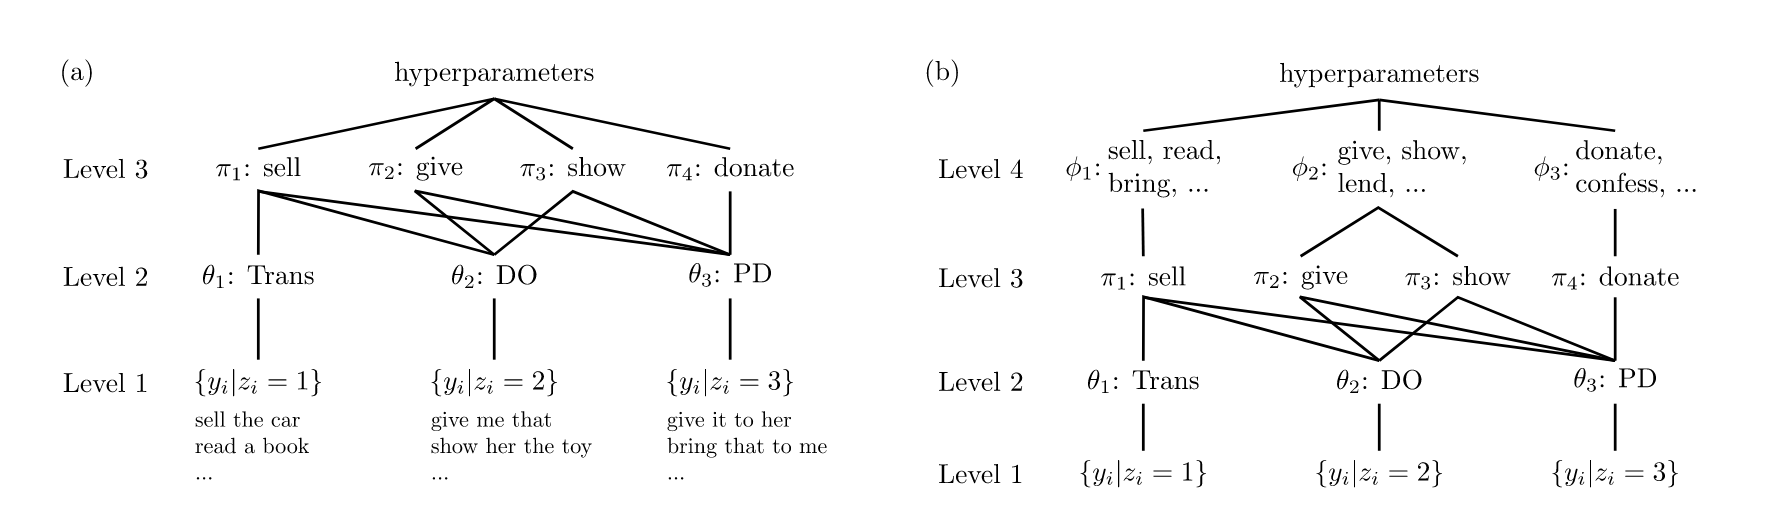
\includegraphics[width=\textwidth]{figures/verb_alternation_classes.png}
    \centering
\end{figure}



\subsection{Cross-lingual verb sense alignment}\label{subsec:verblist}

A cross-lingual aligned list of counterpart verbs will be needed to compare the verb classes and valency frames. The easiest way to do this is likely through existing cross-lingual word lists such as LanguageNet, part of the PanLex project. http://uakari.ling.washington.edu/languagenet/available/

Alternatively, lexicon induction from cross-lingual word embeddings and other NLP methods may also be considered.

\subsection{Information theory}\label{subsec:infotheory}

Complexity and point-wise mutual information, cf. in \citet{say2014}.
Complexity \& Point-wise mutual information (PMI)
\section{Work plan}\label{sec:plan}

This section presents a work plan and the tentative timeline for the thesis project.

\begin{figure}[t]
    \centering
    \begin{adjustbox}{center,scale=0.65}
    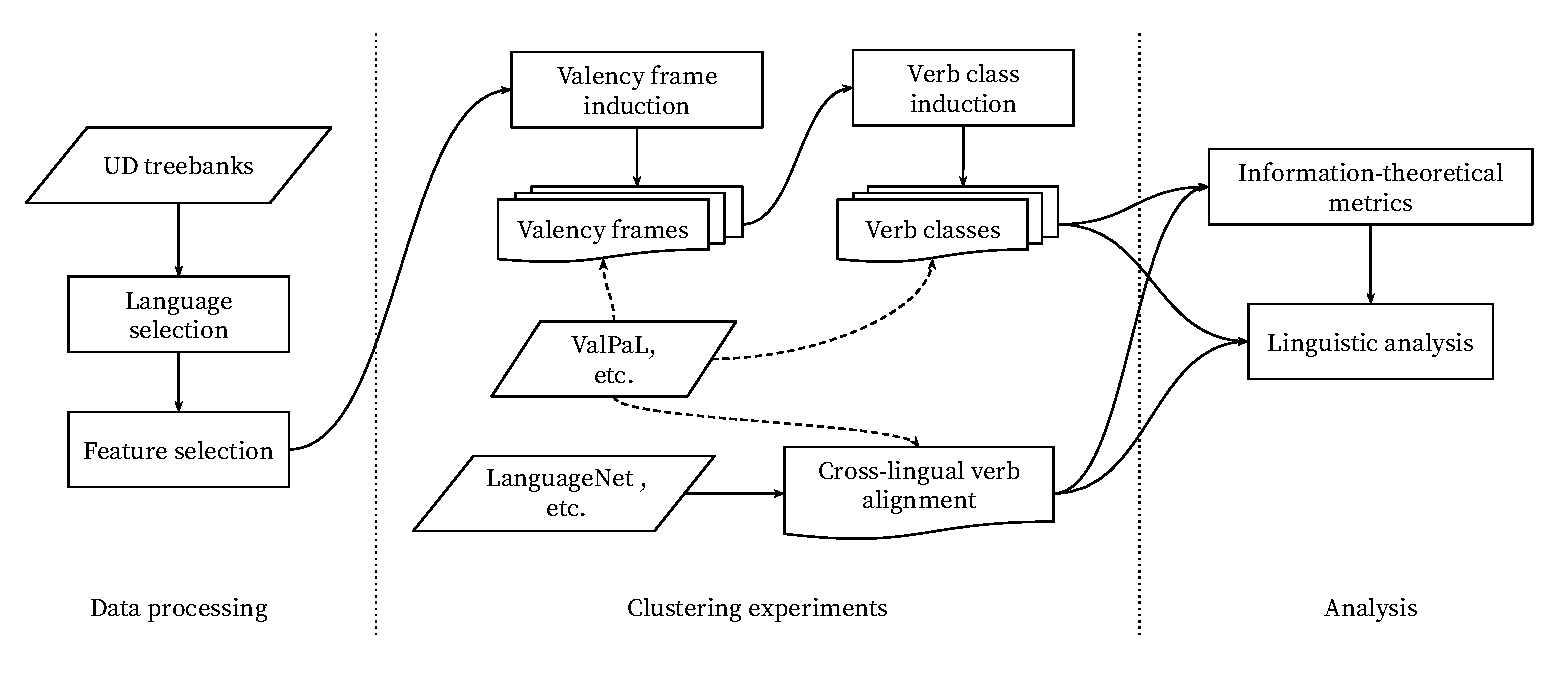
\includegraphics{figures/proposal_flowchart.pdf}
    \end{adjustbox}
    \caption{Flowchart depicting the data sources and processes as described in the proposal. Dotted lines depict validation steps.}\label{fig:flowchart}
\end{figure}

\todo{describe the processes}

This thesis study is intended to be completed within roughly three months after the submission of this proposal, with a statutory maximum of six months.

Given time constraints, an iterative process is envisioned and priority will be put on completing a functional pipeline of the computational part already in the first month of the work, i.e. January, allowing for more flexibility later in the project. Iterative improvements will then be made upon the code and alternate methods tested. The primary experimental parts should conclude by the end of second month to allow for time needed for the write-up and revisions in the final month. 

\section{Conclusion}\label{sec:conclusion}

The proposed thesis would like to contribute to the study of verbal valency systems by including the typological and quantitative perspectives. It will first and foremost attempt novel combinations of computational methods and corpora in service of a quantitative typological investigation, therefore exploring the utility and limits of dependency-based datasets and automatic clustering methods. In doing so, it also aims to contribute to the typological study and theoretical debate on verbal valency. It is hoped that the difficulty in working out a finite categorical typology of valency class systems may be overcome through statistical and information-theoretic methods and modern computational corpora; and that furthermore the empirical study can bring out patterns and observations that may not have been obvious in an introspective study, which may help settle or intensify theoretical debates on valency.

% \citet{levin1993} observed in her study of English verb classes that
% \begin{quote}
%     Distinctions induced by diathesis alternations help to provide insights into verb meaning, and more generally into the organization of the English verb lexicon, that might not otherwise be apparent, bringing out unexpected similarities and differences between verb. (p.15)
% \end{quote}


% \appendix
% \include{appendices/appendix_a}

\newpage
\section*{Bibliography}
\printbibliography[heading=none]
\end{document}
